\section{Tutoriel d'utilisation}
Voici comment utiliser les 3 principales fonctionnalités du projet que sont la création d'une partie, le déroulement de celle-ci (faire bouger et attaquer une unité, terminer un tour, etc) et comment les sauvegarder et charger. 

\subsection{Créer une partie}
\begin{figure}[h]
	\centering
	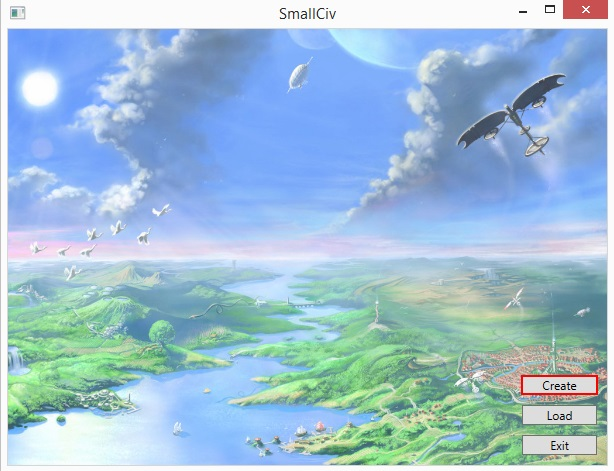
\includegraphics{img/acceuil_to_creation.jpg}
	\caption{L'écran de menu principal du jeu}
	\label{start}
\end{figure}
Au lancement de l'exécutable, l'écran d’accueil s'affichera en fenêtré. Plutôt sobre, il vous permettra de faire 2 actions : créer une nouvelle partie ou en charger une ancienne. Nous allons tout d'abord nous concentrer sur la première d'entre elles. En cliquant sur le bouton \emph{create} (cf. \textsc{figure~\ref{start}} en rouge), vous arrivez à l'écran dédié à la création d'une partie.\newline

\begin{figure}[h]
	\centering
	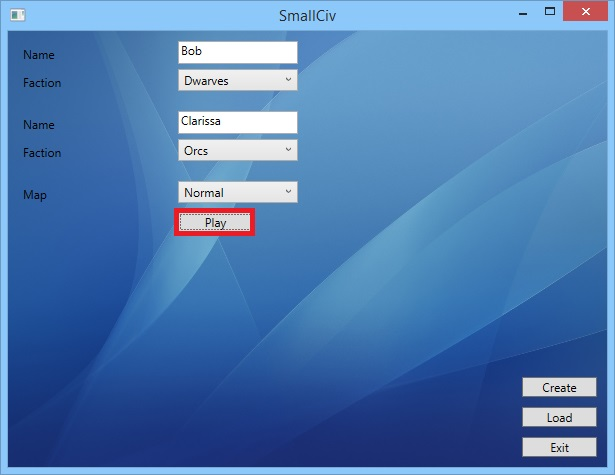
\includegraphics{img/creation.jpg}
	\caption{L'écran de création de partie}
	\label{creation}
\end{figure}
Une fois dans l'écran de création (cf. \textsc{figure~\ref{creation}}), il y a plusieurs choses à faire. Les deux zones \emph{Name} et \emph{Faction} du haut correspondent au nom du joueur 1 et à sa race (elfe nain ou orc, qui sont présentées dans la partie précédente \emph{Règles du jeu}). Les deux champs en-dessous sont leur pendant pour le joueur 2, et enfin le champ \emph{Map} permet de choisir la taille de la carte (démo, petite ou normale, cf \emph{Règles du jeu}).\newline

Ces choix effectués, il ne reste plus qu'à cliquer sur \emph{Play} (en rouge sur la figure) : bien joué, vous avez lancé votre première partie ! 

\subsection{Sauvegarder/charger une partie}
\begin{figure}[h]
	\centering
	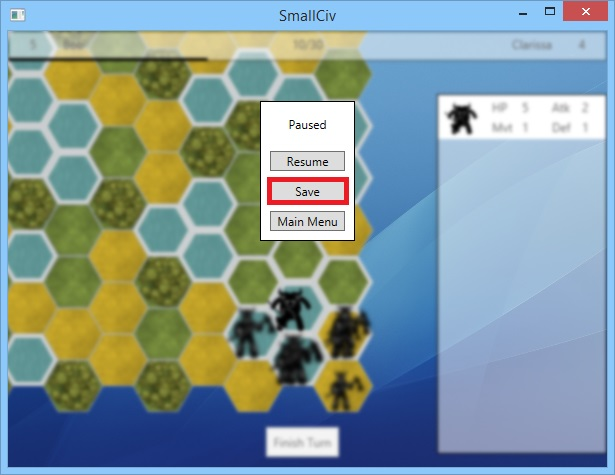
\includegraphics{img/pause_to_save.jpg}
	\caption{L'écran de pause durant une partie}
	\label{pause}
\end{figure}

Voyons tout d'abord comment sauvegarder : quand une partie est en cours, vous pouvez à tout moment appuyer sur \emph{Echap}, cela fait apparaître le menu pause (cf. \textsc{figure~\ref{pause}}). A partir d'ici il vous suffit de cliquer sur \emph{Save} et la partie sera automatiquement sauvegardée. Sauvegarder une partie ne vous fait pas la quitter, aussi le jeu reprend-t-il son cours de suite après. \newline

\begin{figure}[h]
	\centering
	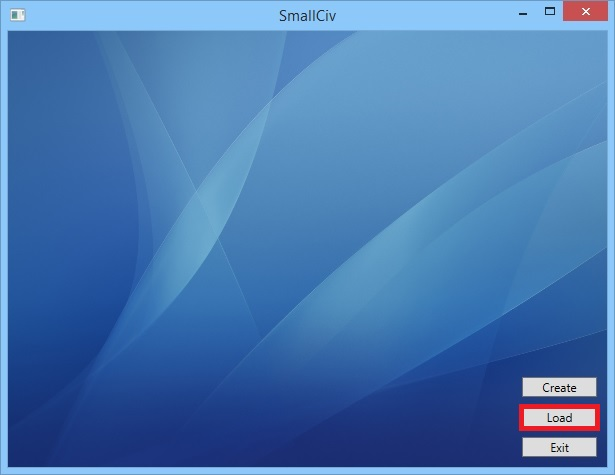
\includegraphics{img/acceuil_to_load.jpg}
	\caption{L'écran de menu principal du jeu}
	\label{start2}
\end{figure}
Le chargement d'une partie se fait à partir de l'écran d’accueil (cf. \textsc{figure~\ref{start2}}) : vous devez cliquer sur \emph{Load} et la dernière partie enregistrée est automatiquement chargée. 

\subsection{Déroulement d'un tour}
\begin{figure}[h]
	\centering
	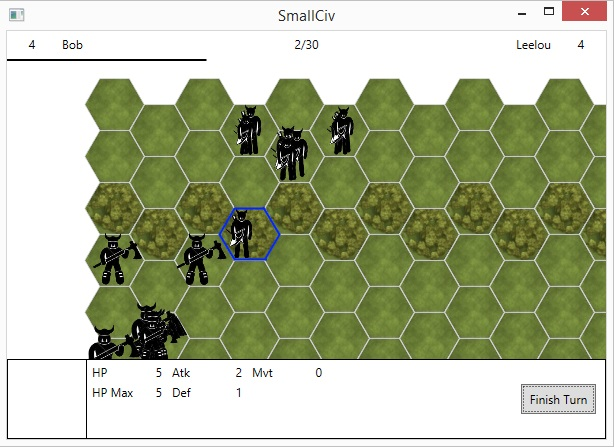
\includegraphics{img/jeu.jpg}
	\caption{Une partie en cours}
	\label{in_game}
\end{figure}
Il y a de nombreuses actions possibles en jeu. Commençons par présenter l'interface utilisateur (cf. \textsc{figure~\ref{in_game}}). La zone de texte représente toutes les unités présentes sur la case avec leurs statistiques ; celle qui va être bougée est mise en évidence. On sélectionne unité \textit{via} un clic gauche sur son sprite à l'écran.\newline

En haut de l'écran on peut voir le score et le pseudo du joueur 1 à gauche (ici, Bob) et ceux du joueur 2 à droite (ici, Leelou). Entre les deux, il s'agit du tour actuel et du nombre de tours maximum de la partie. \newline

Enfin, on déplace l'image pour observer une autre partie de la carte simplement en déplaçant son curseur sur les bordures de la fenêtres pour la faire défiler. \newline

\begin{figure}[h]
	\centering
	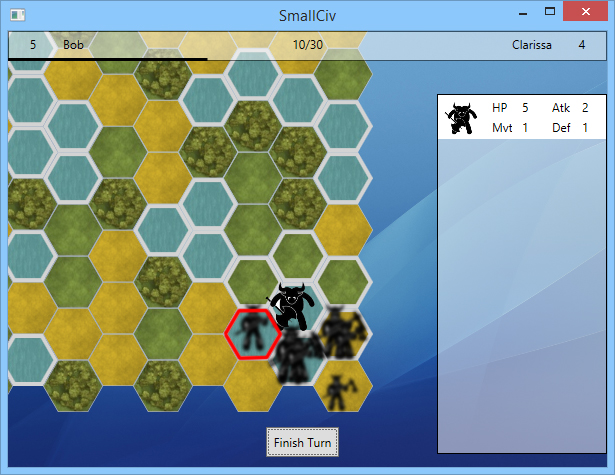
\includegraphics{img/mvt_atk.jpg}
	\caption{Une unité en position d'attaquer}
	\label{mvt_atk}
\end{figure}
Voyons maintenant pour le mouvement et l'attaque. Nous avons dit plus tôt que l'on sélectionnait une unité d'un clic gauche. Sur la \textsc{figure~\ref{mvt_atk}}, c'est au tour de Bob, qui contrôle les elfes, au nord-ouest de la carte. L'unité sélectionnée est celle marquée en bleu, on voit qu'elle a 1 point de déplacement (Mvt).\newline

Elle peut donc au choix se déplacer sur une des tuiles que le jeu met en évidence par une bordure épaisse, ou attaquer l'adversaire sur la tuile rouge qui est à portée. Dans les deux cas, Bob doit faire un clic droit sur sa destination, soit une tuile vide soit la tuile ennemie rouge.\newline

\begin{figure}[h]
	\centering
	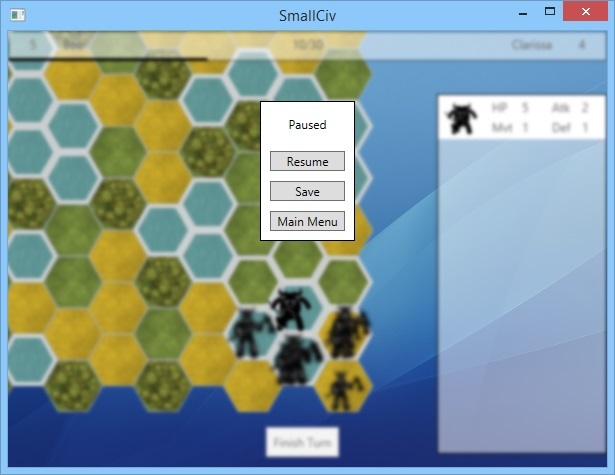
\includegraphics{img/pause.jpg}
	\caption{L'écran de pause durant une partie}
	\label{poause2}
\end{figure}
Le dernier point à aborder dans ces tutoriels est le menu de pause(cf. \textsc{figure~\ref{pause2}}). Nous avons vu plus tôt que le bouton \emph{Save} sauvegarde la partie en cours. Le bouton \emph{Resume} ferme simplement le menu pause et reprend la partie où elle s'était arrêtée, tandis que \emph{Main Menu} termine la partie en cours, la perdant définitivement si elle n'a pas été sauvegardée auparavant, et renvoie au menu principal présenté plus tôt.